\documentclass[fleqn, a4paper. 12pt]{jsarticle} 
\usepackage{cite}
\usepackage{amsmath,txfonts}
\usepackage{amssymb}
\usepackage{url}
\usepackage[margin=31mm]{geometry}
\usepackage[dvipdfmx]{graphicx}
\usepackage{listings,jvlisting}
\usepackage{fancyhdr}
\usepackage{lastpage}
\usepackage{hyperref}
\usepackage[subrefformat=parens]{subcaption}
\lstset{
  basicstyle={\ttfamily},
  identifierstyle={\small},
  commentstyle={\smallitshape},
  keywordstyle={\small\bfseries},
  ndkeywordstyle={\small},
  stringstyle={\small\ttfamily},
  frame={tb},
  breaklines=true,
  columns=[l]{fullflexible},
  numbers=left,
  xrightmargin=0zw,
  xleftmargin=3zw,
  numberstyle={\scriptsize},
  stepnumber=1,
  numbersep=1zw,
  lineskip=-0.5ex
}
\renewcommand{\lstlistingname}{プログラム}

% header
\pagestyle{fancy}
\fancyhf{}
\rhead{2024-05}
\lhead{谷 知拓 - Tomohiro Tani}
\cfoot{\thepage\ / \pageref{LastPage}}

\geometry{left=25mm,right=25mm,top=25mm,bottom=30mm}

\begin{document}

  \begin{titlepage}
    \begin{center}
      {\Huge 2024年度\\応用プログラミング実験}
      
      \vspace{4cm}
      {\Huge 第9-11回\\デジタル信号処理\\
        実験レポート\\
      }
      \vspace{4cm}
      {\large 学修番号: 22140026\\谷 知拓 - Tomohiro Tani\footnote{東京都立大学 システムデザイン学部 情報科学科 \\ mail@taniii.com} \\}
      \vspace{0.5cm}
      {\large
        第1回レポート提出日 : 2024-06-12 \\
      }
    \end{center}
  \end{titlepage}

  \section*{はじめに}

    本レポートでは,『応用プログラミング実験』第9-11回デジタル信号処理の実施報告を行う.

  \subsection*{実験の概要}

    本実験では,デジタル信号処理について学ぶ.
    以下の課題に取り組み,その結果を報告する.

    \begin{enumerate}
      \item 課題1-1: 1Hz 正弦波
      \item 課題1-2: 周波数変化
      \item 課題1-3: 振幅変化
      \item 課題1-4: 周波数および位相変化
      \item 課題1-5: 直流変化
      \item 課題1-6: 信号の加算
      \item 課題1-7: 非周期信号
      \item 課題1-A: 追加課題
    \end{enumerate}

  \subsection*{実験環境}

    実験環境は以下の通りである.

    \begin{itemize}
      \item OS\footnote{Operating System}: macOS Ventura 13.4.1
      \item CPU\footnote{Central Processing Unit}: Apple M2 arm64\footnotemark[4]
      \item メインメモリ・ビデオメモリ共通: 16GBユニファイドメモリ\footnotemark[4]
      \footnotetext[4]{https://www.apple.com/jp/macbook-air-13-and-15-m2/specs/}
      \item 実行環境 (python3): Python 3.12.3
    \end{itemize}

  \newpage
  \section*{課題1-1: 1Hz 正弦波}

    条件は次の通りである.

    \begin{itemize}
      \item $T_0 = 1 [\mathrm{sec}]$
      \item $A = 1$
      \item $\theta = 1 [\mathrm{rad}]$
      \item $D = 0$
    \end{itemize}

    図 \ref{fig:s1} は,周期アナログ信号 $x_{T_0}(t)=A \sin \left(2 \pi F_0 t+\theta\right)+D$ および,その信号を標本化した離散時間信号 $x[n]$ をプロットしたものである.
    
    続いて,離散時間信号 $x[n]$ の離散フーリエスペクトル $X[k]$ を求めた.
    
    図 \ref{fign:a1} は,振幅スペクトル $|X[k]|$ を,図 \ref{fign:p1} は,位相スペクトル $\angle X[k][\mathrm{rad}]$ を示している.

    表 \ref{tab:1} は,周波数インデクス $k$ と各変数の対応表である.

    \begin{figure}[!h]
      \centering
      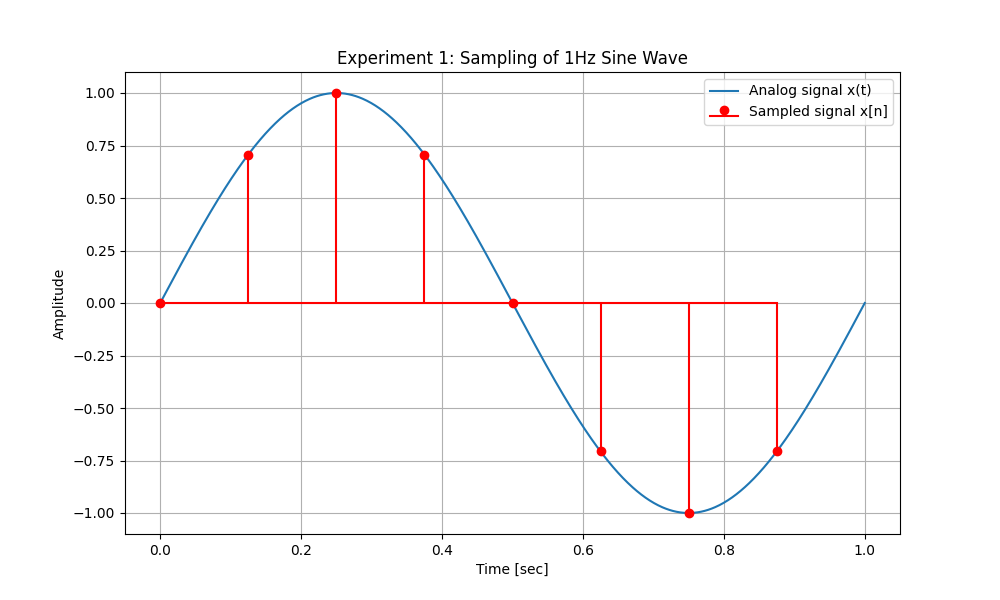
\includegraphics[width=0.6\textwidth]{sampling_experiment_1.png}
      \caption{周期アナログ信号 $x_{T_0}(t)$ とその信号を標本化した離散時間信号 $x[n]$}
      \label{fig:s1}
    \end{figure}

    \begin{figure}[h]
      \begin{center}
      \begin{minipage}[t]{0.48\columnwidth}
          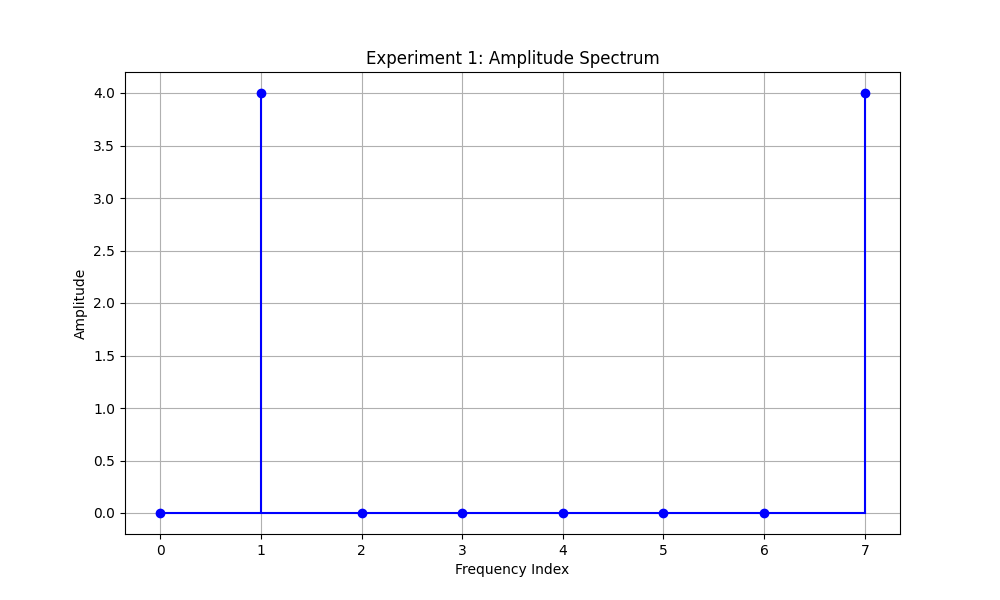
\includegraphics[width=\columnwidth]{amplitude_spectrum_experiment_1.png}
          \subcaption{振幅スペクトル $|X[k]|$}
          \label{fign:a1}
      \end{minipage}
      \begin{minipage}[t]{0.48\columnwidth}
          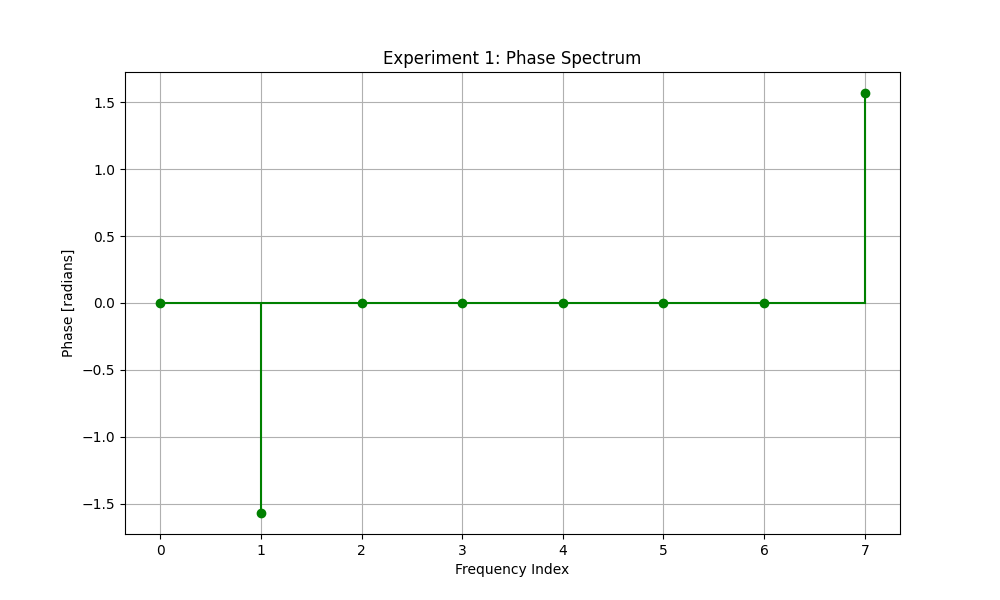
\includegraphics[width=\columnwidth]{phase_spectrum_experiment_1.png}
          \subcaption{位相スペクトル $\angle X[k][\mathrm{rad}]$}
          \label{fign:p1}
      \end{minipage}
      \end{center}
      \caption{離散時間信号 $x[n]$ の離散フーリエスペクトル $X[k]$}
    \end{figure}

    \begin{table}[!h]
      \centering
      \caption{周波数インデクス $k$ と各変数の対応表}
      \begin{tabular}{c|c|c|c|c|c|c|c|c}
        k & 0.0 & 1.0 & 2.0 & 3.0 & 4.0 & 5.0 & 6.0 & 7.0 \\
        \hline
        ω [rad] & 0.000000 & 0.785398 & 1.570796 & 2.356194 & 3.141593 & 3.926991 & 4.712389 & 5.497787 \\
        f & 0.000 & 0.125 & 0.250 & 0.375 & 0.500 & 0.625 & 0.750 & 0.875 \\
        Ω [rad/sec] & 0.000000 & 0.098175 & 0.196350 & 0.294524 & 0.392699 & 0.490874 & 0.589049 & 0.687223 \\
        F [Hz] & 0 & 1 & 2 & 3 & 4 & 5 & 6 & 7 
      \end{tabular}
      \label{tab:1}
    \end{table}

  
  \newpage
  \section*{課題1-2: 周波数変化}

  条件は次の通りである.

  \begin{itemize}
    \item $T_0 = 1/2 [\mathrm{sec}]$
    \item $A = 1$
    \item $\theta = 0 [\mathrm{rad}]$
    \item $D = 0$
  \end{itemize}

  図 \ref{fig:s2} は,周期アナログ信号 $x_{T_0}(t)=A \sin \left(2 \pi F_0 t+\theta\right)+D$ および,その信号を標本化した離散時間信号 $x[n]$ をプロットしたものである.

  続いて,離散時間信号 $x[n]$ の離散フーリエスペクトル $X[k]$ を求めた.

  図 \ref{fign:a2} は,振幅スペクトル $|X[k]|$ を,図 \ref{fign:p2} は,位相スペクトル $\angle X[k][\mathrm{rad}]$ を示している.

  \begin{figure}[!h]
    \centering
    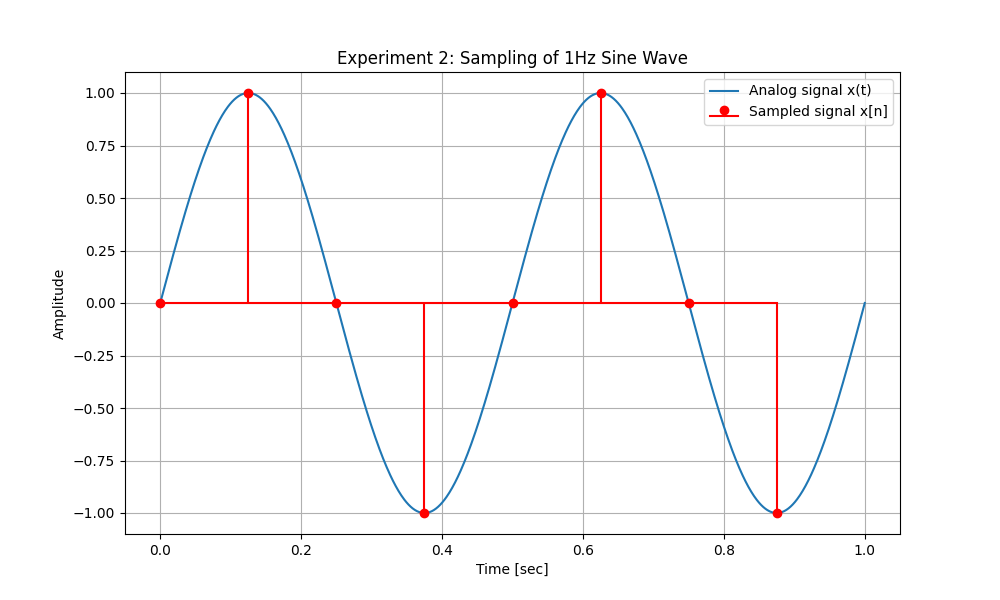
\includegraphics[width=0.6\textwidth]{sampling_experiment_2.png}
    \caption{周期アナログ信号 $x_{T_0}(t)$ とその信号を標本化した離散時間信号 $x[n]$}
    \label{fig:s2}
  \end{figure}

  \begin{figure}[h]
    \begin{center}
    \begin{minipage}[t]{0.48\columnwidth}
        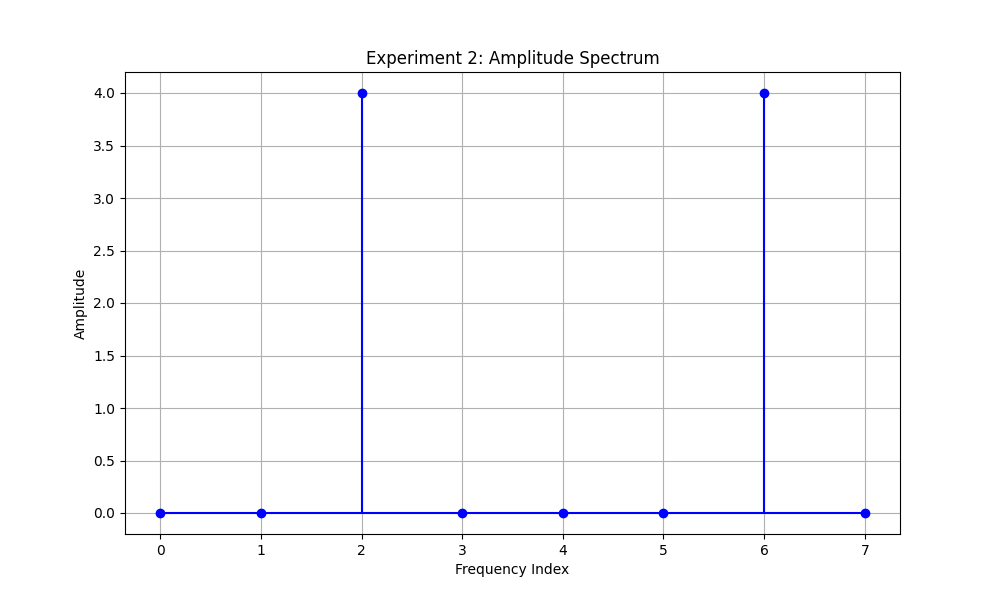
\includegraphics[width=\columnwidth]{amplitude_spectrum_experiment_2.png}
        \subcaption{振幅スペクトル $|X[k]|$}
        \label{fign:a2}
    \end{minipage}
    \begin{minipage}[t]{0.48\columnwidth}
        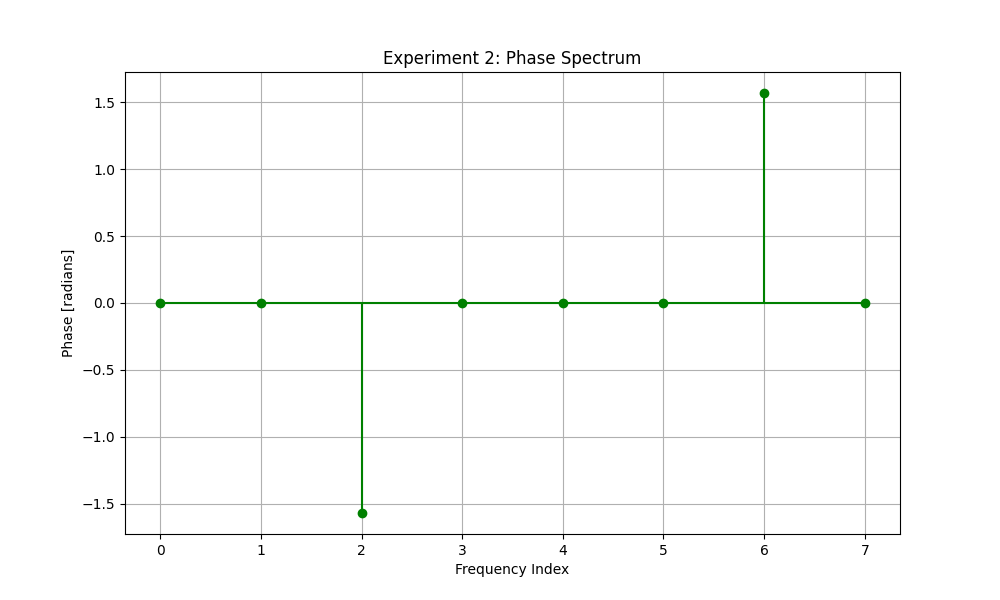
\includegraphics[width=\columnwidth]{phase_spectrum_experiment_2.png}
        \subcaption{位相スペクトル $\angle X[k][\mathrm{rad}]$}
        \label{fign:p2}
    \end{minipage}
    \end{center}
    \caption{離散時間信号 $x[n]$ の離散フーリエスペクトル $X[k]$}
  \end{figure}

  \newpage

  \section*{課題1-3: 振幅変化}
    
  条件は次の通りである.

  \begin{itemize}
    \item $T_0 = 1 [\mathrm{sec}]$
    \item $A = 2$
    \item $\theta = 0 [\mathrm{rad}]$
    \item $D = 0$
  \end{itemize}

  図 \ref{fig:s3} は,周期アナログ信号 $x_{T_0}(t)=A \sin \left(2 \pi F_0 t+\theta\right)+D$ および,その信号を標本化した離散時間信号 $x[n]$ をプロットしたものである.

  続いて,離散時間信号 $x[n]$ の離散フーリエスペクトル $X[k]$ を求めた.

  図 \ref{fign:a3} は,振幅スペクトル $|X[k]|$ を,図 \ref{fign:p3} は,位相スペクトル $\angle X[k][\mathrm{rad}]$ を示している.

  \begin{figure}[!h]
    \centering
    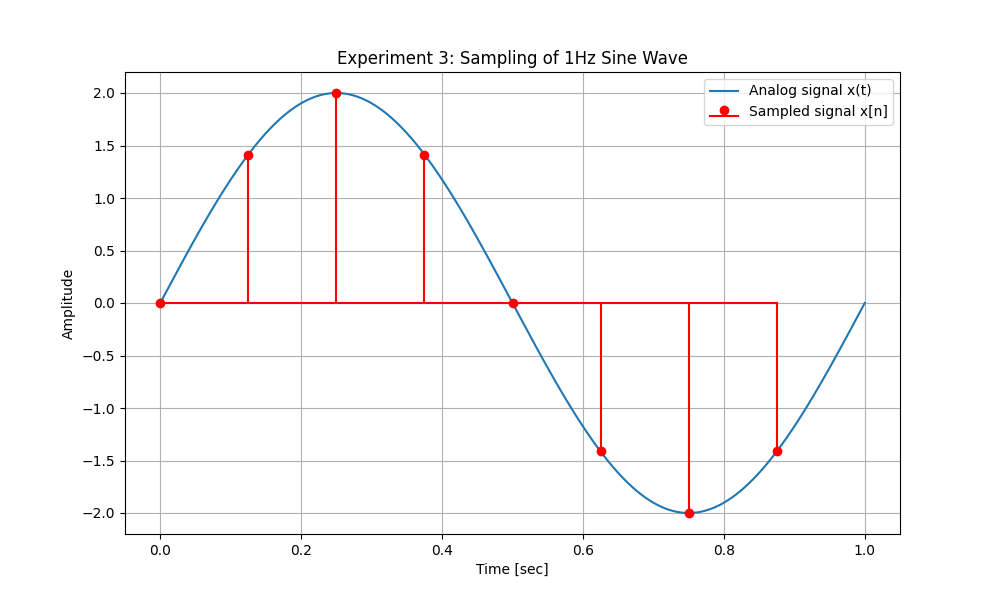
\includegraphics[width=0.6\textwidth]{sampling_experiment_3.png}
    \caption{周期アナログ信号 $x_{T_0}(t)$ とその信号を標本化した離散時間信号 $x[n]$}
    \label{fig:s3}
  \end{figure}

  \begin{figure}[h]
    \begin{center}
    \begin{minipage}[t]{0.48\columnwidth}
        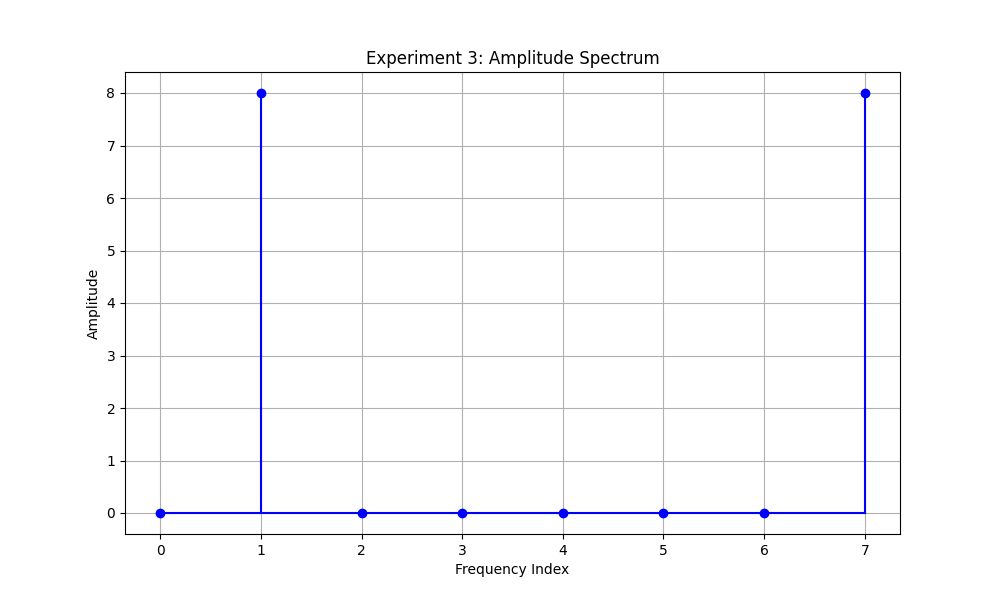
\includegraphics[width=\columnwidth]{amplitude_spectrum_experiment_3.png}
        \subcaption{振幅スペクトル $|X[k]|$}
        \label{fign:a3}
    \end{minipage}
    \begin{minipage}[t]{0.48\columnwidth}
        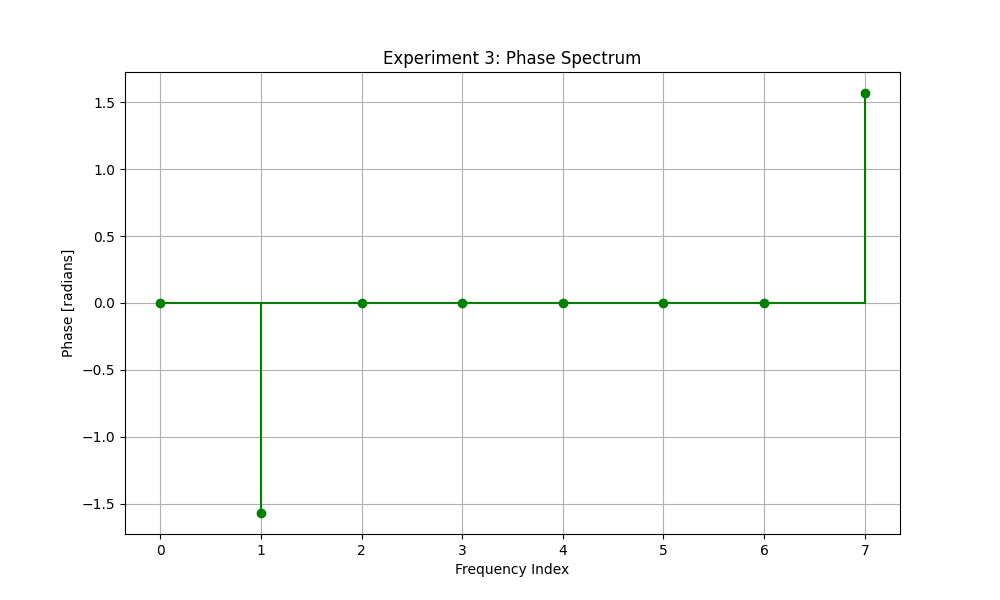
\includegraphics[width=\columnwidth]{phase_spectrum_experiment_3.png}
        \subcaption{位相スペクトル $\angle X[k][\mathrm{rad}]$}
        \label{fign:p3}
    \end{minipage}
    \end{center}
    \caption{離散時間信号 $x[n]$ の離散フーリエスペクトル $X[k]$}
  \end{figure}

  \newpage

  \section*{課題1-4: 周波数および位相変化}

  条件は次の通りである.

  \begin{itemize}
    \item $T_0 = 1/2 [\mathrm{sec}]$
    \item $A = 1$
    \item $\theta = \pi [\mathrm{rad}]$
    \item $D = 0$
  \end{itemize}

  図 \ref{fig:s4} は,周期アナログ信号 $x_{T_0}(t)=A \sin \left(2 \pi F_0 t+\theta\right)+D$ および,その信号を標本化した離散時間信号 $x[n]$ をプロットしたものである.

  続いて,離散時間信号 $x[n]$ の離散フーリエスペクトル $X[k]$ を求めた.

  図 \ref{fign:a4} は,振幅スペクトル $|X[k]|$ を,図 \ref{fign:p4} は,位相スペクトル $\angle X[k][\mathrm{rad}]$ を示している.

  \begin{figure}[!h]
    \centering
    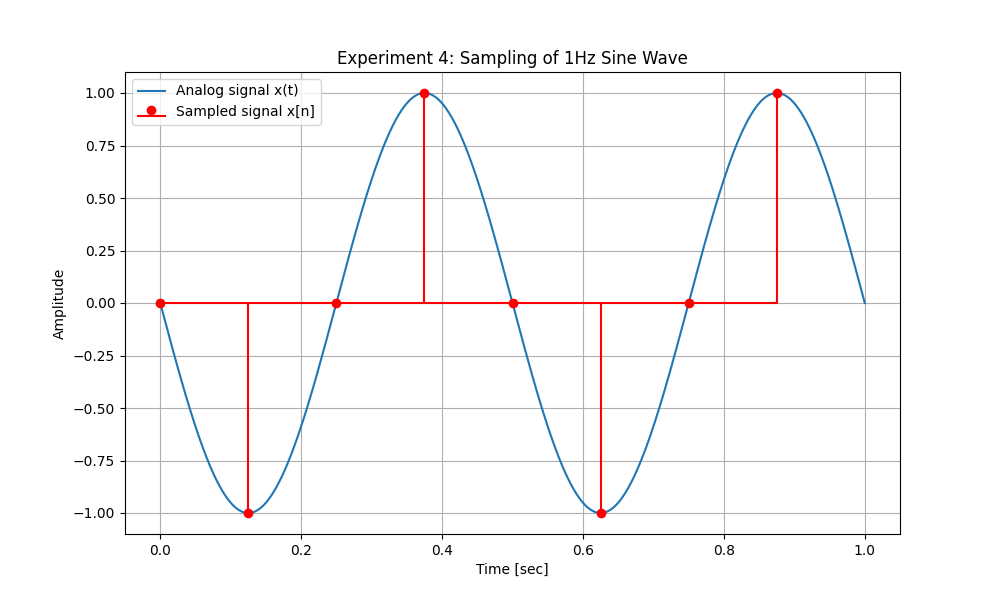
\includegraphics[width=0.6\textwidth]{sampling_experiment_4.png}
    \caption{周期アナログ信号 $x_{T_0}(t)$ とその信号を標本化した離散時間信号 $x[n]$}
    \label{fig:s4}
  \end{figure}

  \begin{figure}[h]
    \begin{center}
    \begin{minipage}[t]{0.48\columnwidth}
        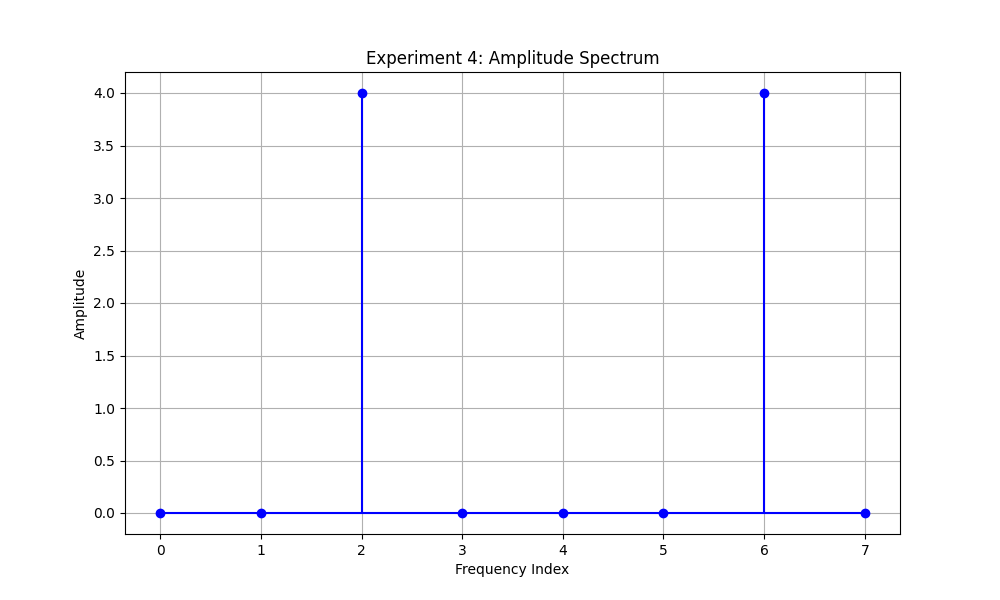
\includegraphics[width=\columnwidth]{amplitude_spectrum_experiment_4.png}
        \subcaption{振幅スペクトル $|X[k]|$}
        \label{fign:a4}
    \end{minipage}
    \begin{minipage}[t]{0.48\columnwidth}
        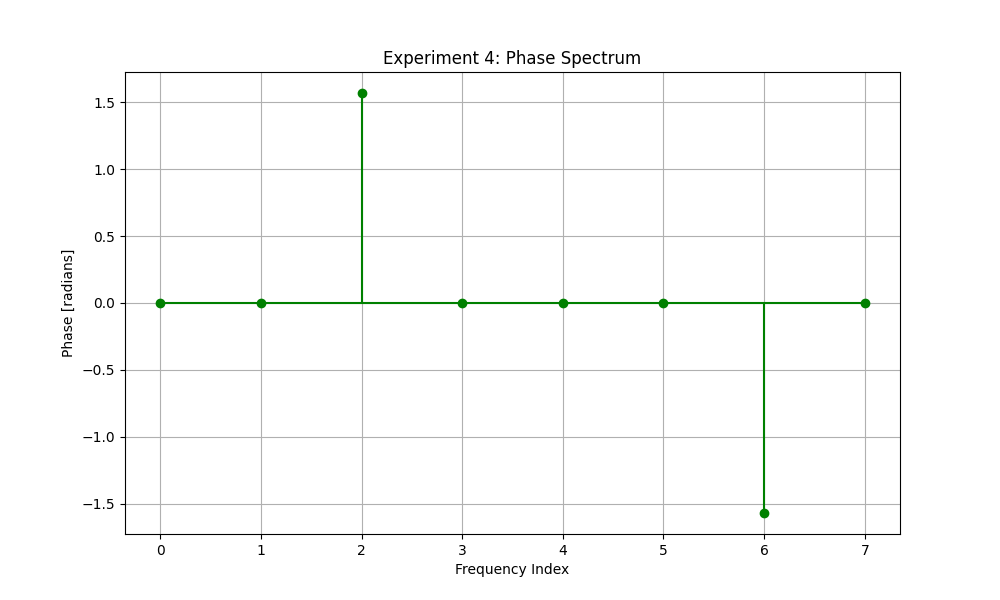
\includegraphics[width=\columnwidth]{phase_spectrum_experiment_4.png}
        \subcaption{位相スペクトル $\angle X[k][\mathrm{rad}]$}
        \label{fign:p4}
    \end{minipage}
    \end{center}
    \caption{離散時間信号 $x[n]$ の離散フーリエスペクトル $X[k]$}
  \end{figure}

  \newpage

  \section*{課題1-5: 直流変化}

  条件は次の通りである.

  \begin{itemize}
    \item $T_0 = 1 [\mathrm{sec}]$
    \item $A = 1$
    \item $\theta = 0 [\mathrm{rad}]$
    \item $D = 1$
  \end{itemize}

  図 \ref{fig:s5} は,周期アナログ信号 $x_{T_0}(t)=A \sin \left(2 \pi F_0 t+\theta\right)+D$ および,その信号を標本化した離散時間信号 $x[n]$ をプロットしたものである.

  続いて,離散時間信号 $x[n]$ の離散フーリエスペクトル $X[k]$ を求めた.

  図 \ref{fign:a5} は,振幅スペクトル $|X[k]|$ を,図 \ref{fign:p5} は,位相スペクトル $\angle X[k][\mathrm{rad}]$ を示している.

  \begin{figure}[!h]
    \centering
    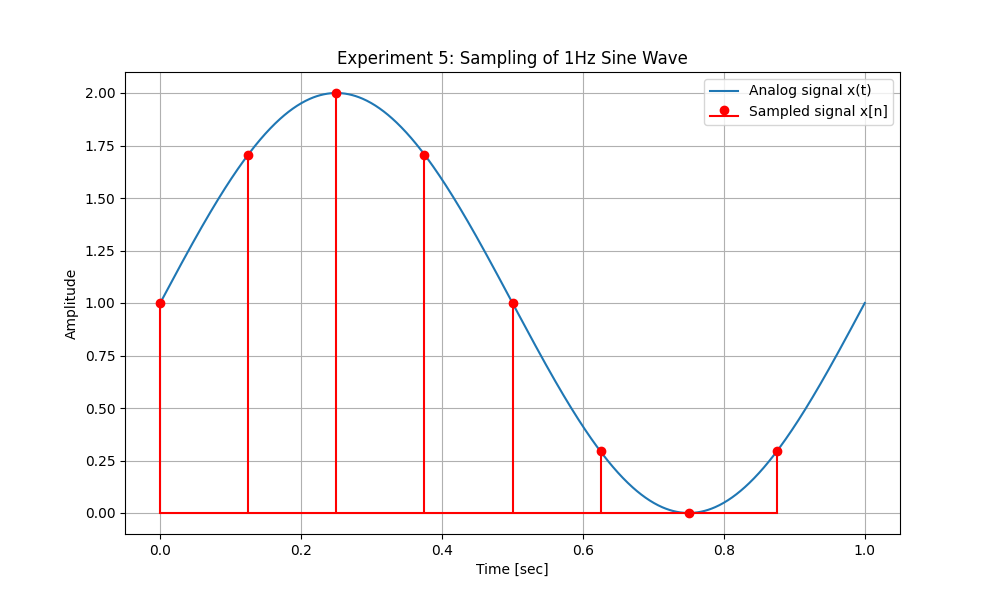
\includegraphics[width=0.6\textwidth]{sampling_experiment_5.png}
    \caption{周期アナログ信号 $x_{T_0}(t)$ とその信号を標本化した離散時間信号 $x[n]$}
    \label{fig:s5}
  \end{figure}

  \begin{figure}[h]
    \begin{center}
    \begin{minipage}[t]{0.48\columnwidth}
        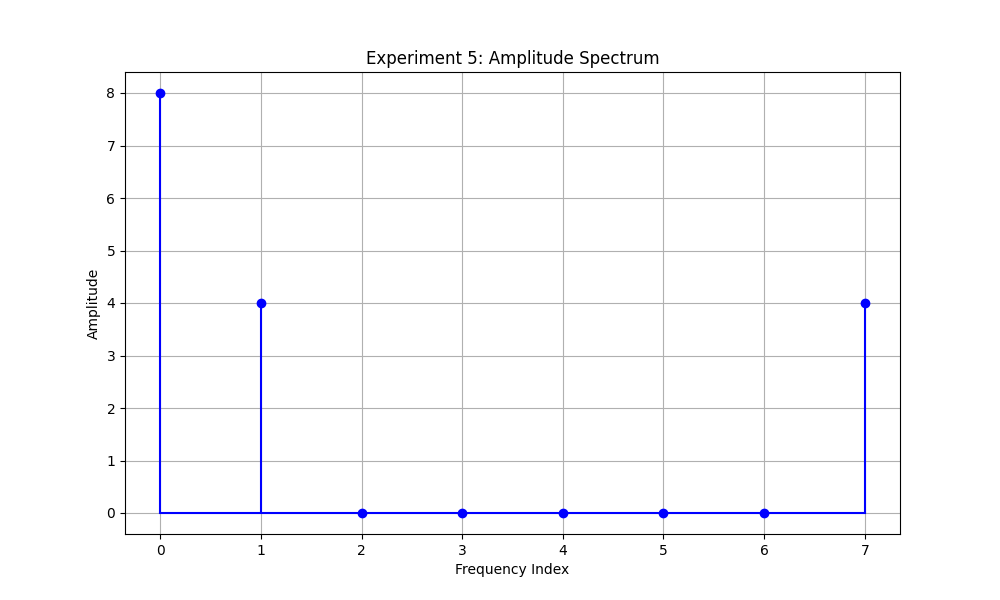
\includegraphics[width=\columnwidth]{amplitude_spectrum_experiment_5.png}
        \subcaption{振幅スペクトル $|X[k]|$}
        \label{fign:a5}
    \end{minipage}
    \begin{minipage}[t]{0.48\columnwidth}
        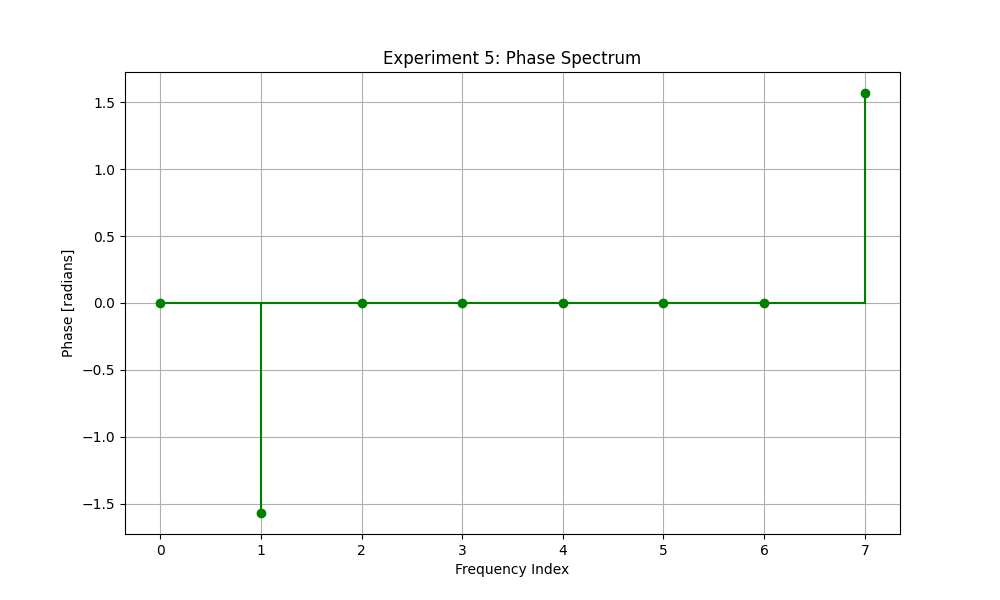
\includegraphics[width=\columnwidth]{phase_spectrum_experiment_5.png}
        \subcaption{位相スペクトル $\angle X[k][\mathrm{rad}]$}
        \label{fign:p5}
    \end{minipage}
    \end{center}
    \caption{離散時間信号 $x[n]$ の離散フーリエスペクトル $X[k]$}
  \end{figure}

  \newpage

  \section*{課題1-6: 信号の加算}

  条件は次の通りである.

  \begin{itemize}
    \item $T_0 = 1 [\mathrm{sec}]$
  \end{itemize}

  図 \ref{fig:s6} は,周期アナログ信号 $a_{T_0}(t)=2 \sin (2 \pi t)+\sin (4 \pi t+\pi)$ および,その信号を標本化した離散時間信号 $a[n]$ をプロットしたものである.

  続いて,離散時間信号 $a[n]$ の離散フーリエスペクトル $X[k]$ を求めた.

  図 \ref{fign:a6} は,振幅スペクトル $|X[k]|$ を,図 \ref{fign:p6} は,位相スペクトル $\angle X[k][\mathrm{rad}]$ を示している.

  \begin{figure}[!h]
    \centering
    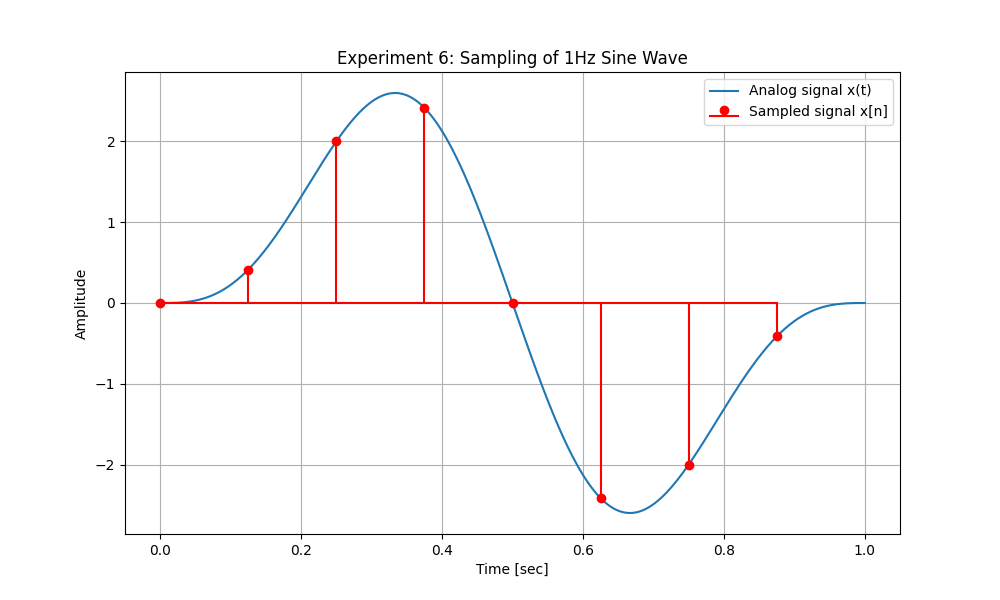
\includegraphics[width=0.6\textwidth]{sampling_experiment_6.png}
    \caption{周期アナログ信号 $x_{T_0}(t)$ とその信号を標本化した離散時間信号 $x[n]$}
    \label{fig:s6}
  \end{figure}

  \begin{figure}[h]
    \begin{center}
    \begin{minipage}[t]{0.48\columnwidth}
        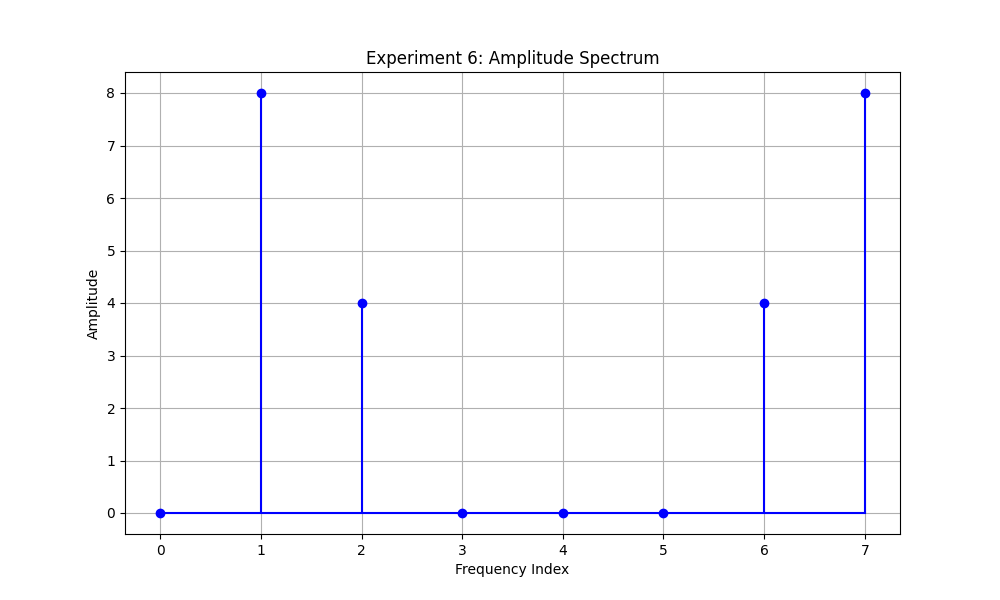
\includegraphics[width=\columnwidth]{amplitude_spectrum_experiment_6.png}
        \subcaption{振幅スペクトル $|X[k]|$}
        \label{fign:a6}
    \end{minipage}
    \begin{minipage}[t]{0.48\columnwidth}
        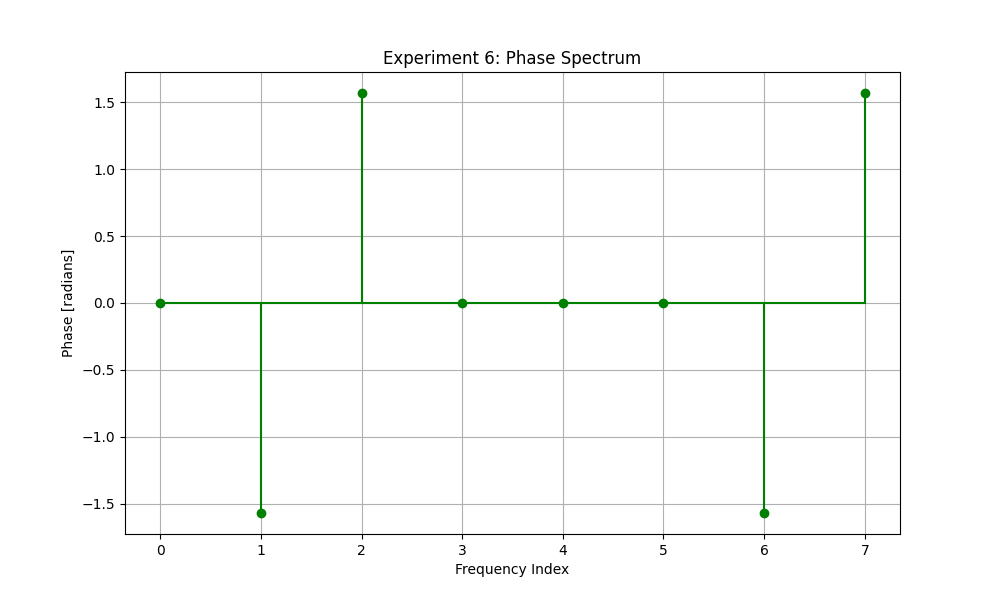
\includegraphics[width=\columnwidth]{phase_spectrum_experiment_6.png}
        \subcaption{位相スペクトル $\angle X[k][\mathrm{rad}]$}
        \label{fign:p6}
    \end{minipage}
    \end{center}
    \caption{離散時間信号 $x[n]$ の離散フーリエスペクトル $X[k]$}
  \end{figure}

  \newpage

  \section*{課題1-7: 非周期信号}

  条件は次の通りである.

  \begin{itemize}
    \item $T_0 = 0.8 [\mathrm{sec}]$
    \item $A = 1$
    \item $\theta = 1 [\mathrm{rad}]$
    \item $D = 0$
  \end{itemize}

  図 \ref{fig:s7} は,周期アナログ信号 $x_{T_0}(t)=A \sin \left(2 \pi F_0 t+\theta\right)+D$ および,その信号を標本化した離散時間信号 $x[n]$ をプロットしたものである.
  
  続いて,離散時間信号 $x[n]$ の離散フーリエスペクトル $X[k]$ を求めた.
  
  図 \ref{fign:a7} は,振幅スペクトル $|X[k]|$ を,図 \ref{fign:p7} は,位相スペクトル $\angle X[k][\mathrm{rad}]$ を示している.

  \begin{figure}[!h]
    \centering
    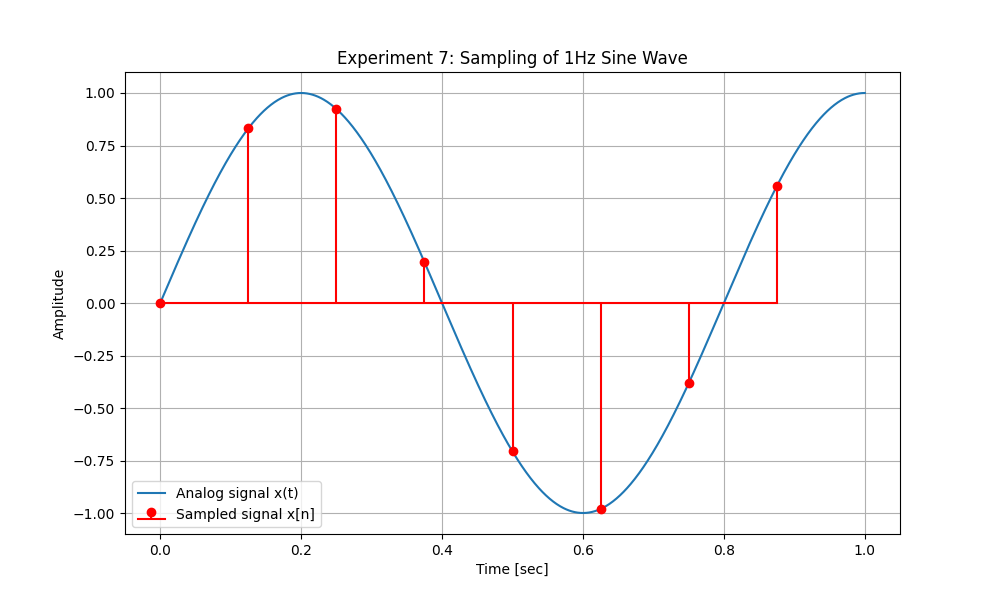
\includegraphics[width=0.6\textwidth]{sampling_experiment_7.png}
    \caption{周期アナログ信号 $x_{T_0}(t)$ とその信号を標本化した離散時間信号 $x[n]$}
    \label{fig:s7}
  \end{figure}

  \begin{figure}[h]
    \begin{center}
    \begin{minipage}[t]{0.48\columnwidth}
        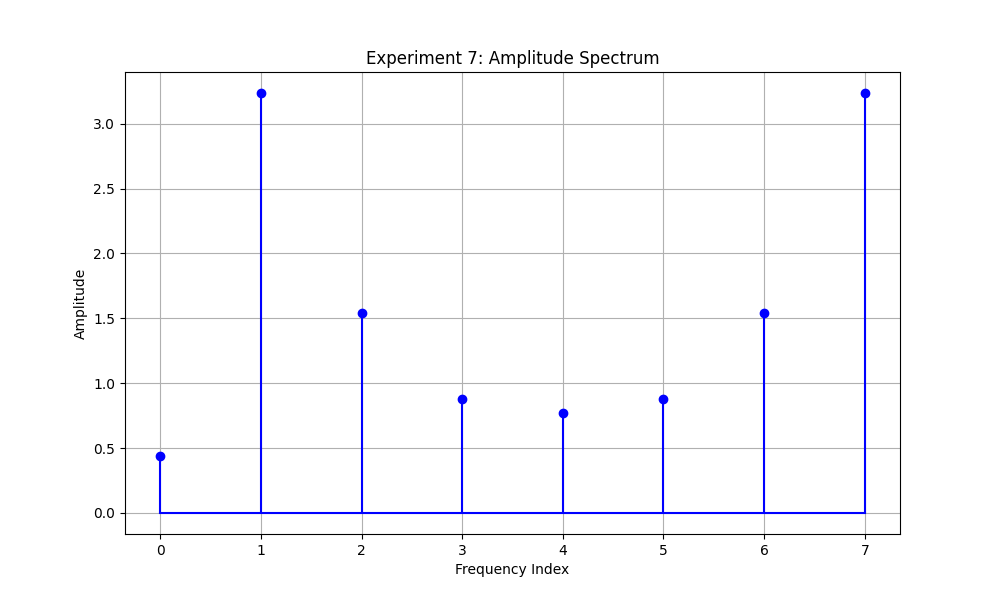
\includegraphics[width=\columnwidth]{amplitude_spectrum_experiment_7.png}
        \subcaption{振幅スペクトル $|X[k]|$}
        \label{fign:a7}
    \end{minipage}
    \begin{minipage}[t]{0.48\columnwidth}
        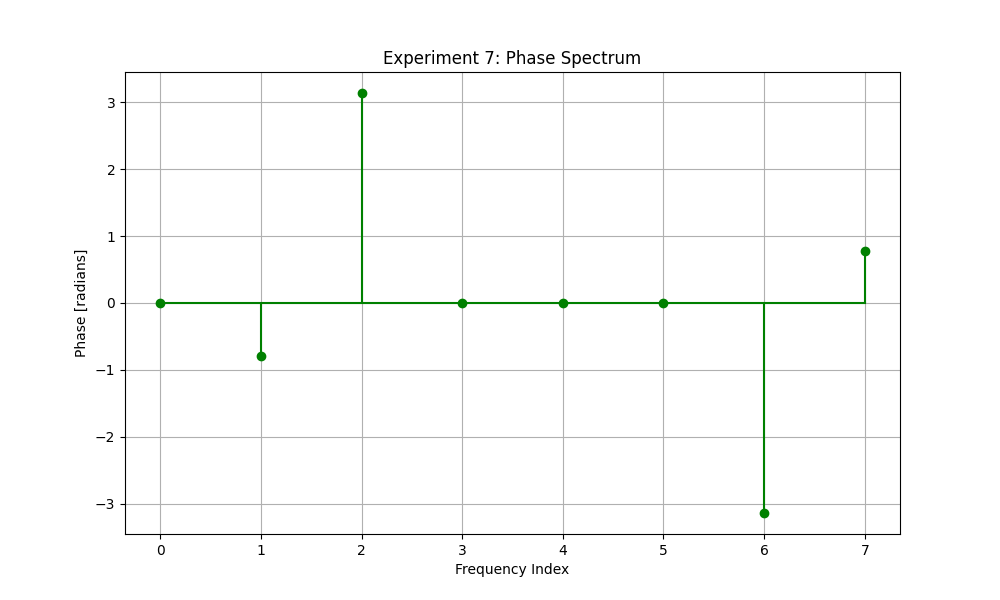
\includegraphics[width=\columnwidth]{phase_spectrum_experiment_7.png}
        \subcaption{位相スペクトル $\angle X[k][\mathrm{rad}]$}
        \label{fign:p7}
    \end{minipage}
    \end{center}
    \caption{離散時間信号 $x[n]$ の離散フーリエスペクトル $X[k]$}
  \end{figure}

  \newpage

  \section*{おわりに}

    第1回では,様々なシミュレーションをコンピュータを用いて行うには,期待する分布に従った乱数生成の手法が必要不可欠であることがわかった.
    
    また,乱数生成の品質がシミュレーション結果に大きな影響を与えるということを理解することができた.

    \quad

    第2回では,生成したイベントの発生回数の確率分布が,理論値とくるいなく一致しているのが印象的であった.

    世界のさまざまな事象をモデル化するのに,確率分布という概念が非常に重要であることがわかった.

    \quad

    第3回では,待ち行列のモンテカルロシミュレーションを行うことができ,特に Queue を用いた非同期処理システムをモデル化できたのがとても興味深かった.

    現在,開発業で,分散型メールシステムに関わる非同期処理システムの構築を行なっているため,今回の課題は非常に参考になった.

    具体的には,メールサーバからの取得プロトコルである,IMAP は 40 年近く前の 1986 年に誕生したため,現代の Webhook のようなステートレスにイベントを受け取る仕組みが十分でなく,最新のメールが来ていないかどうか,メールアカウントごとに確認しにいく必要があり,ここに非同期の待ち行列モデルが生じるため,設計に試行錯誤している.

  \newpage
  
  \section*{参考文献}

    \begin{itemize}
        \item Learn Rust - Rust Programming Language: \url{https://www.rust-lang.org/learn} (accessed: May 22, 2024)
    \end{itemize}

    \begin{itemize}
      \item Kleinrock, Leonard (1975). "Queueing Systems Volume 1: Theory"
    \end{itemize}

\end{document}